\documentclass[tightenline,notitlepage,nofootinbib]{revtex4-1}

\bibliographystyle{plainnat}
%\DeclareOption{nofootinbib}{\@booleanfalse\footinbib@sw}

%\@booleanfalse\footinbib@sw

\usepackage{graphicx}
\usepackage{amsmath}
\usepackage{subcaption}
\usepackage{sidecap}
\usepackage{empheq}


\DeclareMathOperator{\erf}{Erf}
\DeclareMathOperator{\trace}{Tr}

\newcommand{\spinup}{\uparrow}
\newcommand{\spindown}{\downarrow}
\newcommand{\KSAE}{{I}}
\newcommand{\qav}[1]{\langle {#1} \rangle}
\newcommand*{\ket}[1]{\left \lvert {#1} \right \rangle}
\newcommand*{\bra}[1]{\left \langle {#1} \right \rvert}
\newcommand{\comm}[1]{{ \textbf{#1} }}



\begin{document}
  \title{An upgrade study of chargino detection with finer mass splittings.}
  \author{Janis Erdmanis \\ graphitewriter@gmail.com}
%  \email{akels14@gmail.com}
  \date{August 2016}
  \maketitle

  \section{Introduction}

  In the standart model Higgs mass is highly sensitive to the details of the physics at high-energy [...]. Unless we accept big number cancelactions in SM, it does not work well with naturalness principle and so we may find solution in BSM physics. One of theories which resolves this issue is supersimetry which introduces new particles, new processes at higher energies. Present knowledge of exlcluded susy parameters requires small higsino mass splittings with energies larger than $100 GeV$\footnote{From data of Large electron positron accelerator.}, but smaller than $1 TeV$ for naturalness principle to hold. This study considers possibility to catch susy signal in high luminosity LHC data from ATLAS experiment with higsino mass splittings $\Delta m = 5 GeV$ and $\mu=100 GeV$ (see figure).
%  mass splittings for higgsino particles which we are trying to catch here with assumption that we would have high luminosity LHC data from ATLAS experiment.

  In our study we are trying to find signal which comes from $pp$ colision produced chargaino particle $\tilde \chi_1^{+},\tilde \chi_1^{-}$ decay to $W$ and $Z$ bosons and further to two or three measurable soft leptons and neitrinos and neitralinos (see figure). If in the $pp$ collision also single jet is produced then for conserving transverse momentum a big missing energy would be produced for neitrinos and neitralinos which will distinguish singnal from standart model background.
  \begin{figure}[!ht]
    \centering
    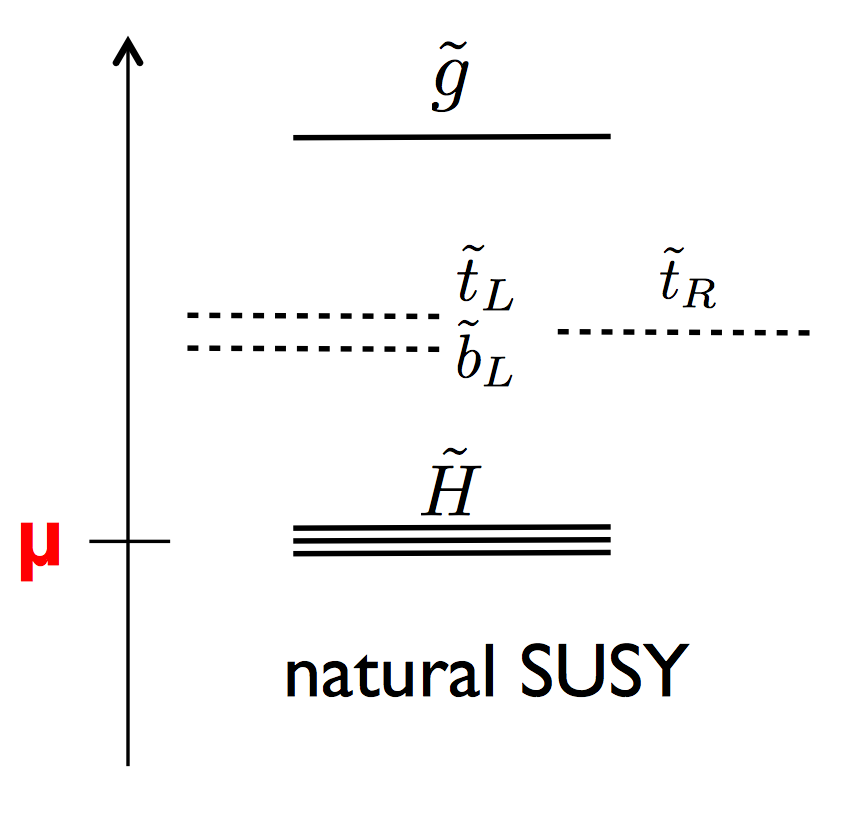
\includegraphics[width=0.25\textwidth]{splittings.png}
    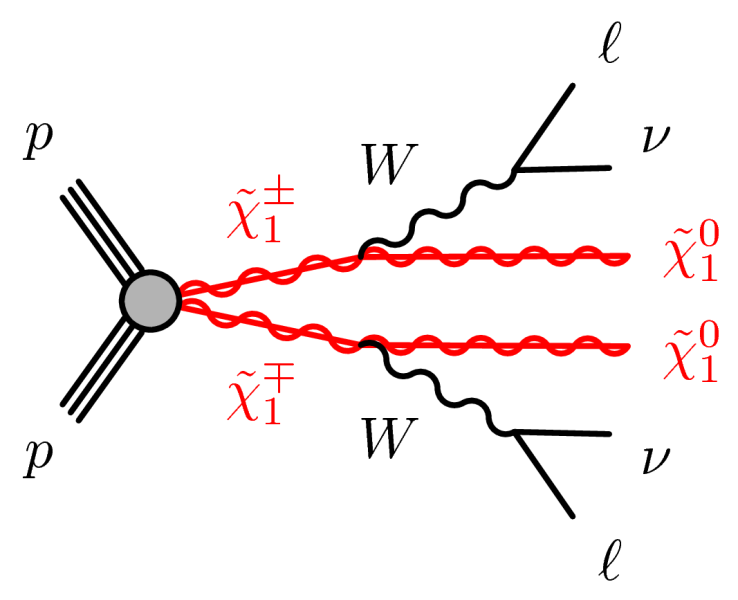
\includegraphics[width=0.25\textwidth]{C1C1.png}
    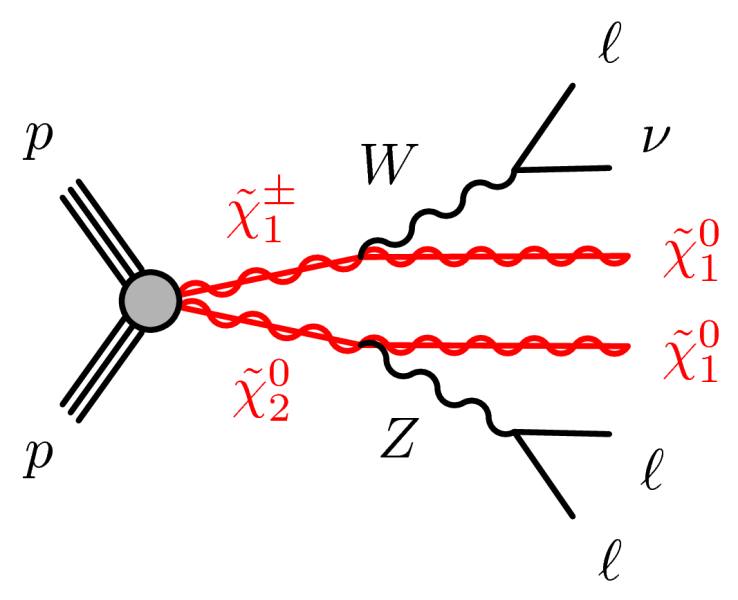
\includegraphics[width=0.25\textwidth]{C1N2.png}
    \caption{Considered susy signals in our analysis.}
  \end{figure}
 As a background we consider processes $pp\rightarrow \tau \tau + j$, $pp\rightarrow t \bar t + j$, $pp \rightarrow WW + j$. Also because of the large crossection (see table) of process $pp \rightarrow W +j$, we consider also background leptons which are incorectly detected and comes from jets (fake leptons). 
\begin{table}[!ht]
  \centering
  \begin{tabular}{ll}
    Process & $\sigma_{eff}$ \\
    \hline
    $pp\rightarrow \tau \tau + j$ & $47.6 pb$\\
    $pp\rightarrow t \bar t + j$ & $ 8.9pb$\\
    $pp \rightarrow W + j$ &  $162pb$ \\
    $pp \rightarrow WW +j$ & $1.34 pb$\\
    $pp \rightarrow \tilde \chi_1^{+}\tilde \chi_1^{-} + j \rightarrow WW + j$ & $2.8pb$\\
    $pp \rightarrow \tilde \chi_1^{+}\tilde \chi_2^{0} + j \rightarrow WZ + j$ & $5pb$\\
  \end{tabular}
  \caption{Cross sections for considered processes for collisions at $14 TeV$}
\end{table}
% MadGraph event generator for all theese processes is used from which we try to extract signal with appropriate selection.

To study and compare the signal and backgrounds, we turn to Monte Carlo. We simulate the hard processes
for the signal in Eq. (8) and the major backgrounds with Madgraph 6. The parton-level events are then showered and hadronized with Pythia 8. 

\section{Smearing of events}

Because detector simulation is costly we use a simplified detector algorithm. Firstly we smear energies, masses, momenta, $\eta$, $\phi$ of all objects (particles and jets) with corresponding performance functions. As jets also produce leptons we add fake electrons which takes into account performance of jet reconstruction algorithms. At the next step we filter out particles which can be detected in ATLAS - $|\eta_l|<2.5$, $Pt_j>50 GeV$. (What does OverlapRemovel do?). To remove electrons which could come from jets we require that energy and momentum of leptons should be at least $15\%$ with respect to energy of $20^0$ and momentum of $30^0$ cone. Also we remove low mass lepton pairs $m_{ll}<12 GeV$ because .... And lastly we apply $0.9$ probability to actually detect the particle.

To test if the smearing of events works we plotted leading jet transverse momentum at different stages of algorithm (see figure ...). In the figure we see that smearing indeed makes distribution broader, considerable amount of fake particles also are added, and overlap removal helps to recover the shape of generator Pt shape. 
\begin{figure}[!ht]
  \centering
  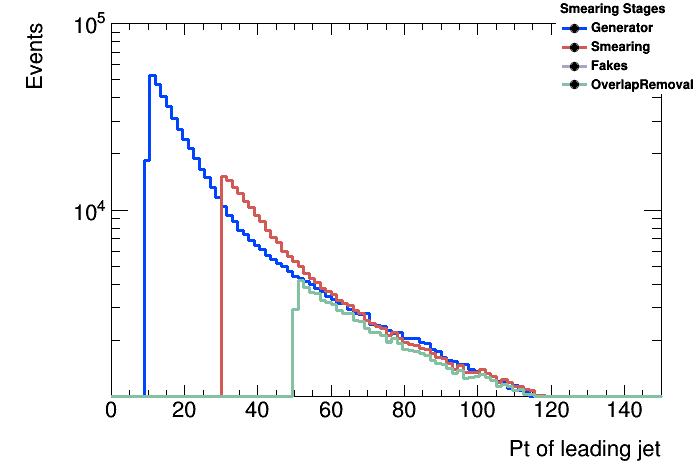
\includegraphics[width=0.45\textwidth]{h_PtJets1stStages.png}
  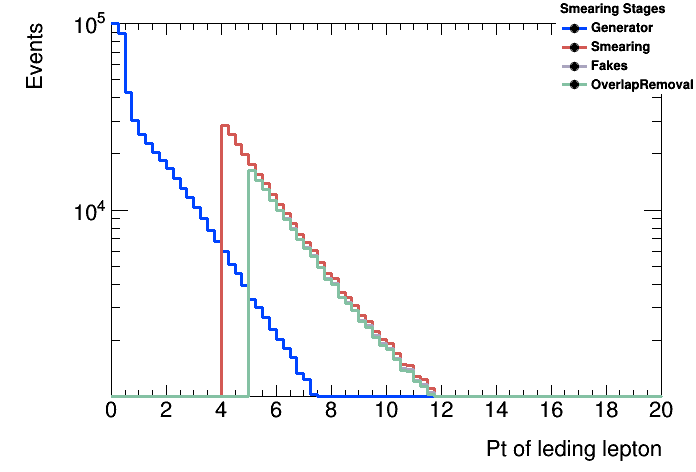
\includegraphics[width=0.45\textwidth]{h_PtEleMuo1stStages.png}
  \caption{Tests of smering functions for signal sample}
\end{figure}

% \begin{figure}[!ht]
%   \centering
%   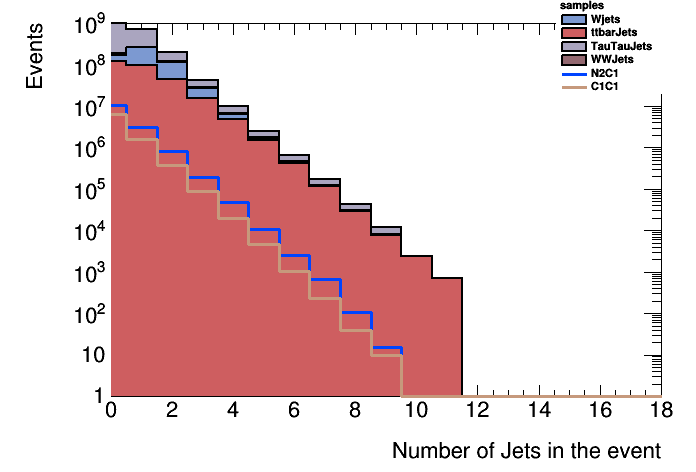
\includegraphics[width=0.25\textwidth]{h_NJet.png}
%   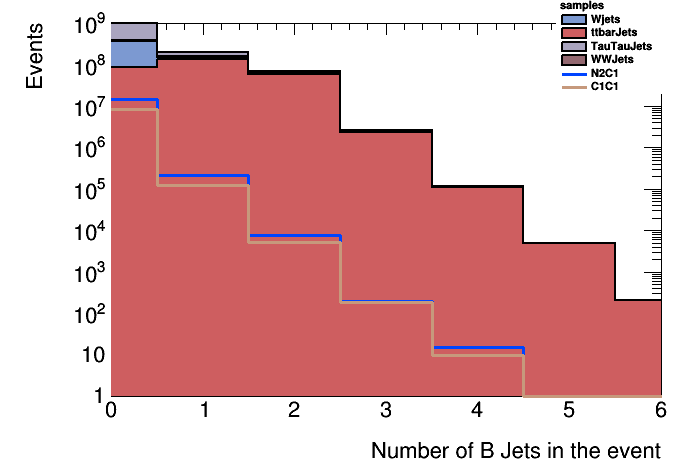
\includegraphics[width=0.25\textwidth]{h_NBJet.png}
%   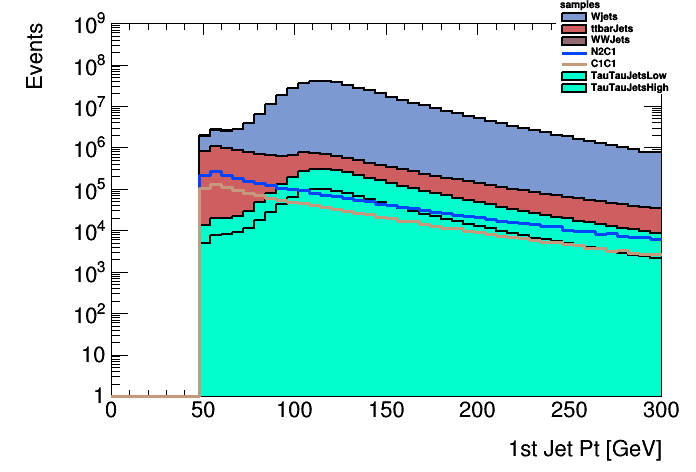
\includegraphics[width=0.25\textwidth]{h_PtJets1st.png}
%   \caption{Number of Jets, Bjets and leading jet transverse momentum.}
% \end{figure}

\section{Event selection}


\begin{figure}[!ht]
  \centering
  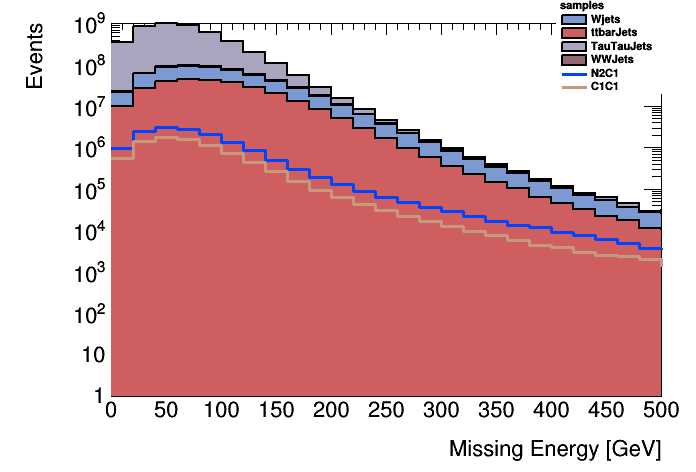
\includegraphics[width=0.3\textwidth]{h_MET.png}
  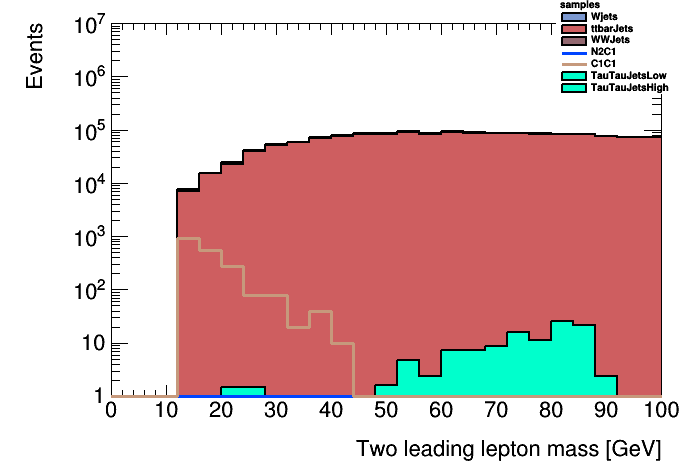
\includegraphics[width=0.3\textwidth]{h_llmass.png}
  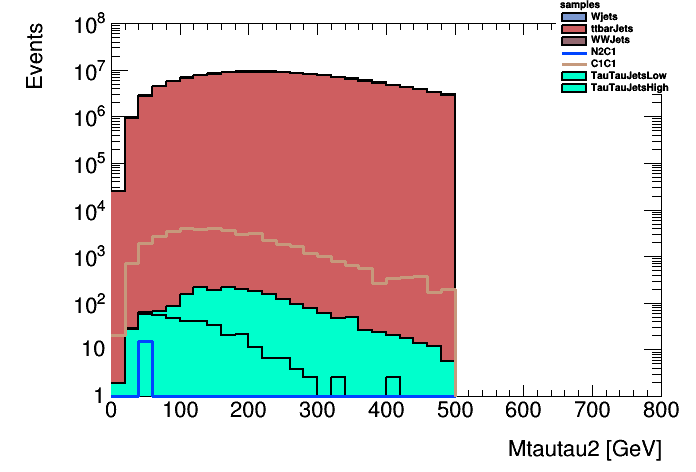
\includegraphics[width=0.3\textwidth]{h_Mtautau2.png}
  \caption{Missing energy, two leading lepton mass $m_{ll}$ and reconstructed tautau mass $m_{\tau\tau}$ with formula (...)}
\end{figure}

To compare and check our simulation and smearing algorithm we use selection from [...] for the same kind of process.  
\begin{itemize}
\item $MET>100 GeV$. Because we expect large missing energy in form of neitralinos and neitronos in our signal.
\item Single Jet with $Pt>100GeV$ and no $Bjets$ in event. We want missing energy to come from particles not in jets and bjets are produced mainly by background $pp->t \bar t + j$.
\item $2~ leading ~ lepton ~ Pt > 7 GeV$. We are eliminating here not considered background
\item $m_{\tau \tau}>150 GeV$. Should eliminate $pp\rightarrow \tau \tau$ background as it has resonance at $100 GeV$. 
\item $M(1st l + 2nd l)<12 GeV$.
\end{itemize}
where we also afterwards make seperation for two and three lepton processes. 

\begin{figure}[!ht]
  \centering
  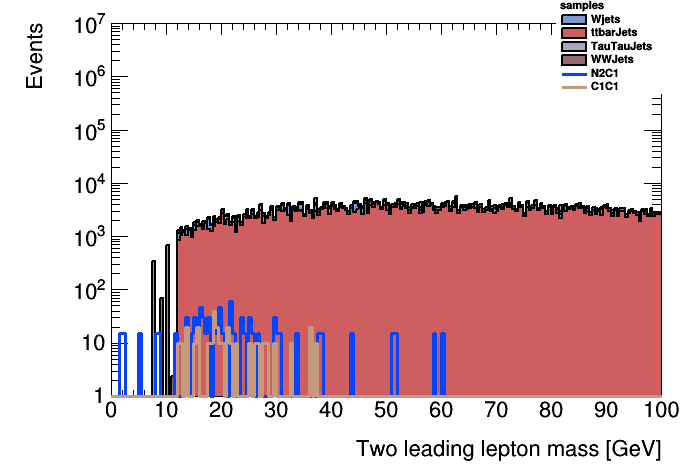
\includegraphics[width=0.45\textwidth]{h_llmass_cuts.png}
  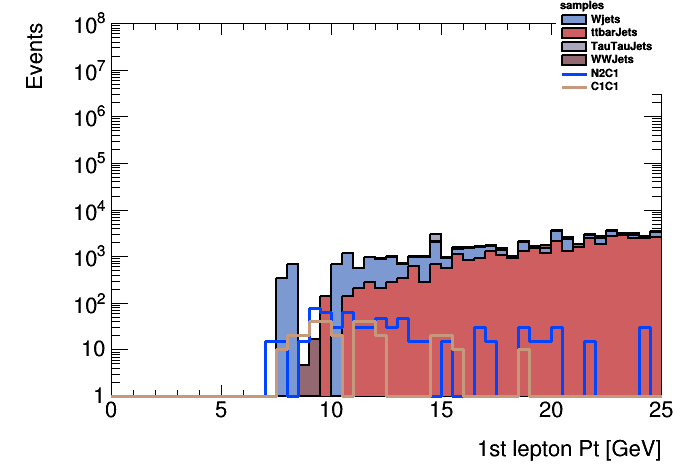
\includegraphics[width=0.45\textwidth]{h_PtMuons1st_cuts.png}
  \caption{The signal after sellection}
\end{figure}


\section{Conclussions}


     
%     \begin{SCfigure}[][p]
%       	 \includegraphics[width=0.6\textwidth]{./Plots/Dispersion_packet_plot}  \caption{The spread of wave packet as function of speed at which energy in quantum dot is raised.}
%     	\label{fig:spread}
%     \end{SCfigure}
  
  
%  \begin{figure}[p]
%  	\begin{subfigure}[b]{0.45\textwidth}
%  	\includegraphics[width=1.1\textwidth]{Plots/Convergence_discreditation.pdf}
%  	\end{subfigure} ~
%  	\begin{subfigure}[b]{0.45\textwidth}
%  	  	\includegraphics[width=1.1\textwidth]{Plots/Convergence_localisation.pdf}
%  	  	\end{subfigure} 
%  	\\
%  	  	\begin{subfigure}[b]{0.45\textwidth}
%  	  	\includegraphics[width=1.1\textwidth]{Plots/Convergence_energy_discreditation.pdf}
%  	  	\end{subfigure}
%  	  	~
%  	    	\begin{subfigure}[b]{0.45\textwidth}
%  	    	\includegraphics[width=1.1\textwidth]{Plots/Convergence_energy_localisation.pdf}
%  	    	\end{subfigure}
%  	\caption{At the top we see direct comparison with time probability distribution obtained from Wigner function with parameters $A_\Gamma=2$, $\tau/\tau_0=2$ numerically by applying property \eqref{asymptotics:time_prob} and also analytically  from kinetic equation \eqref{kinetic} which was taken from \cite{Arnis}. It shows fast convergence as spacing of $T$ becomes smaller than $2 \tau_0/\tau$ at numerical evaluation of integral \eqref{harmonic:Wigner_bar} with trapezoidal rule. The asumption of localisation for integration variable $T$ however does not show signs in time probability distribution (as expected), while in energy probability distribution we see that localisation parameter $a$ must be choosen with respect to normalization $P_{Norm} = \int_{- a/2}^{+a/2} p_t(t) dt$.}
%  	\label{fig:convergence}
%  \end{figure}
  
  
  % ---Bibliography --- 
  \clearpage
  \bibliography{bibliography}{}
%  \bibliographystyle{plain}
  
  
  \end{document}

%%% Local Variables:
%%% mode: latex
%%% TeX-master: t
%%% End:
